\documentclass[a4paper,10pt]{article}

\usepackage[utf8]{inputenc}
\usepackage{graphicx}

\title{SDSS Celestial Objects Classification}
\author{Andrea Sessa Mat.850082}

\begin{document}

\maketitle

\begin{abstract}
  Given the high dimensionality of the data provided by the Spectra instrumentation; main goal of the project
  is to provide a classfication of the celestial object observed by Spectra focusing on the data visualization 
  and features selection phase.\newline
  Various different feautures selection tecnique are evaluated(Principal Component Anaysis(PCA), Kernel PCA, forward features selection,
  backward features selection). The different approaches are compared over a `state-of-the-art` classifier(Support Vector Machine)\newline
  Final results shows that (TODO)
\end{abstract}

\newpage

\tableofcontents

\newpage

\listoffigures

\newpage

\section{Introduction}
  Modern astronomy is concerned with the study of very distant celestial objects ie quasars, galaxies, stars, etc.\newline
  Often this type of classfication is performed by analyzing the spectrum emitted by such objects.\newline
  In general the emission spectrum of a chemical element or of a chemical compound is defined as the eletromagnetic radiation emitted
  when an atom or a molecule, of the object that we are observing, perform a transition from an high energy states to a low energy state.
  During the decadiment the atom or molecule the elettromagnetic is iradiated under the form of photon, the associated photon energy
  (also called flux) is proportional is equal to the energy difference between the two energy states involved in the decadiment.\newline
  The important element is that for a given atom there are many possible electron transition, and each of these transition has a specific
  flux associated.\newline
  The Sloan Digital Sky Survey(henceforth referred as SDSS) is a major imaging and spectroscopic survey using a dedicated 2.5-m wide-angle
  optical telescope at Apache Point Observatory in New Mexico, United States.\newline
  The collection of data started in 2000 and continues up to nowdays(latest data realease in June 2013). The dataset comprises almost
  2 millions of spectra coming from diffrent objects.\newline
  Machine learning plays an important role in the task of classifying these objects, given the fact that many times samples include
  more than 1000 features.\newline
  Features in general includes information about the flux associated with a specific wavelenght.
  \begin{figure}[!ht]
    \caption{Typical emission spectrum for a galaxy}
    \centering
    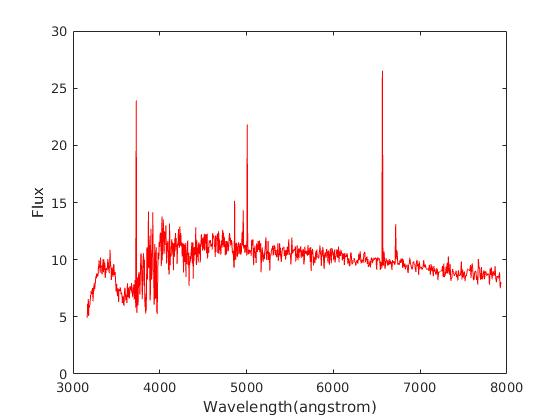
\includegraphics[scale=0.55]{emission_galaxy.jpg}
  \end{figure}
  
  The problem of feautures selection become very important in this scenario; this project will try to cast
  some light on the problem by evaluating different approaches over a reducted version of the SDSS dataset.
  
\newpage

\section{Problem Formulation}

\subsection{Dataset}
  Write something about the dataset, number of samples, number of features, labels, in source 


\section{Methodology}

\section{Experiments}

\section{Conclusions}

\begin{thebibliography}{9}
  \bibitem{spectrum}
    Wikipedia,
    \emph{Emission Spectrum}
    
   \bibitem{sdss}
    Wikipedia,
    \emph{The Sloan Digital Sky Survey}  
\end{thebibliography}


\end{document}
